We rethink the IDE from the group up using a problem-solving perspective to guide our design.
We chose a cards-based metaphor (see Figure~\ref{mockup}) as the basis for the user interface of our IDE.
We briefly highlight and describe five key elements of our design, and indicate their relationship with the previously described challenges.

\begin{itemize}
	\item Cards are containers for different logical elements needed during problem-solving sessions.
	They can contain anything that can be materialized in the pursuit of a solution to a programming problem; i.e., issue tracker cards for individual GitHub issues (\textit{Card 1}), 
	\item 
\end{itemize}

We use Code Bubbles~\cite{bragdon2010bubbles}, Code Canvas~\cite{deline2010canvas}, and Patchworks Code Editor~\cite{henley2014patchworks} as key inspirations for interface designs that eschew window-based interfaces and explore spatial interfaces allowing users to project meaning onto the layout of their development environment.
We also rely upon Lighthouse~\cite{dasilva2006lighthouse} as an inspiration for parallel development awareness in interface design.
Extending the zoomable canvas of Code Canvas and the bubble windows of Code Bubbles, plus the live information of Lighthouse, we explore these and other concepts from interface design to support the problem-solving activities that programmers encounter.

\vspace*{-0.3\baselineskip}
\begin{figure}[h!]
	\caption{Cards-based User Interface of a Problem-Solving IDE}
	\label{mockup}
    \centering
	% trim={<left> <lower> <right> <upper>}	
    \fbox{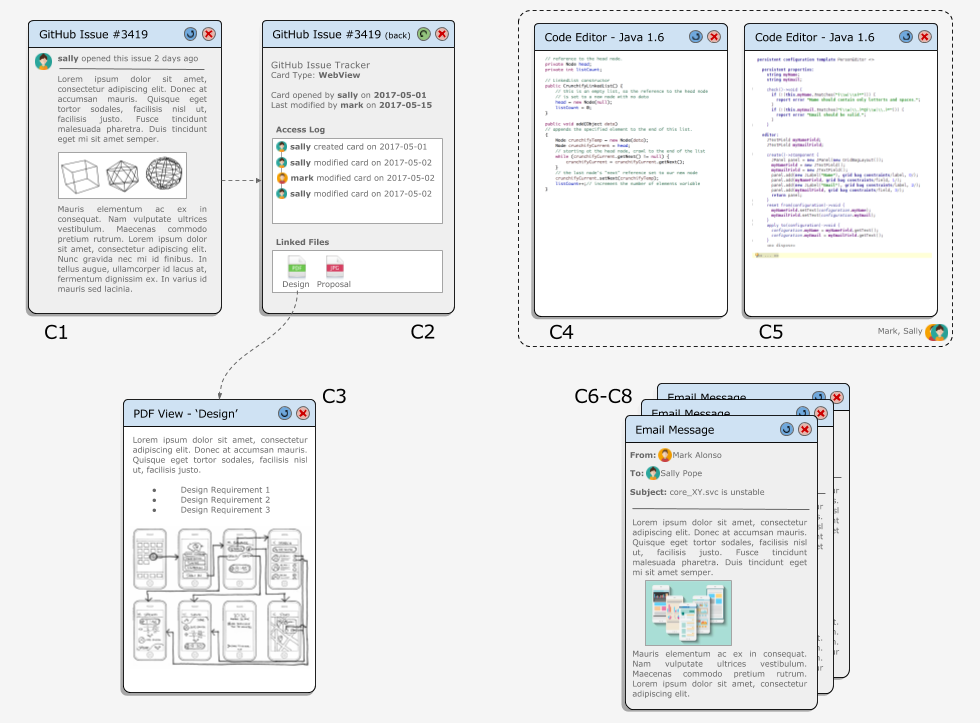
\includegraphics[trim={0.6cm 0.2cm 0.6cm 0.2cm},clip,width=0.9\textwidth]{Mockup-10}}
	\vspace*{-0.4\baselineskip}
\end{figure}

Figure~\ref{mockup} provides a high-fidelity illustration of our proposed user interface for a new IDE that allows user-driven problem-solving to occur natively within a single environment.
As shown in Figure~\ref{mockup}, we propose a cards-based user interface so that developers can take advantage of the neuro-cognitive process of perceptual organization~\cite{kimchi2003perceptual}.
Spatial perception allows developers to provide meaning to individual artifacts (i.e., cards) by organizing them in patterns that contextualize the individual artifact, its relation to other artifacts, and the larger purpose.
As previously demonstrated, developers work with artifacts beyond code and therefore require cards that accommodate those non-code artifacts.
We propose cards of different types to address different problem-solving aspects: code editor cards for code artifacts (cards \texttt{C4}, \texttt{C5}), issue tracker cards for problem contextualization (\texttt{C1}, \texttt{C2}), image and PDF cards for design documents (\texttt{C3}), or email viewer cards for communications (\texttt{C6-C8}).
This list is not exhaustive, and we expect that additional card types will be proposed and developed to accommodate additional problem-solving activities.

Individual cards can be stacked together into logical units of meaning based upon the programming problem and the developer's approach to it (e.g. cards \texttt{C6-C8}).
This flexibility allows cards of different types to be stacked into groups that are relevant to the current task, and then unstacked and stacked again for subsequent tasks.
Since developers work together, in a variety of different capacities (see Table~\ref{pps_matrix} -- A5), we also propose integrated methods for sharing individual cards (or stacks of cards) for either review or simultaneous editing.
This feature can be seen in cards ~\texttt{C4} and \texttt{C5}, which are shown as being shared between two different developers to allow them to discuss and modify the cards as needed to address a programming problem.

Our proposed cards-based IDE attempts to address each of the six problem-solving activities (Table~\ref{pps_matrix}) through the use of cards that allow for the construction and interpretation of artifacts related to the situation (A1), the creation of new contextually relevant cards (A2), the organization of cards in stacks to explore and refine solutions (A3), the ability to directly edit code and other artifacts (A4), the ability to share and synchronization development between individual developers (A5), and to reflect upon and preserve desirable solutions (A6).